\documentclass[a4paper]{report}
\usepackage{setspace}
%\usepackage{subfigure}

% Page styling
\pagestyle{plain}
\usepackage{amssymb,graphicx,color}
\usepackage{amsfonts}
\usepackage{latexsym}
\usepackage[a4paper, margin = 3cm, bottom = 2.5cm]{geometry}

\usepackage{changepage}

% Tables
\usepackage{multirow, multicol}
\setlength{\columnsep}{1cm}

% Custom theorems
\usepackage[font=small, labelfont=bf]{caption}
\usepackage[protrusion=true, expansion=true]{microtype}
\usepackage{sectsty}
\usepackage{url, lipsum}
\usepackage{amsthm}

\usepackage{hyperref}

\theoremstyle{definition}
\newtheorem{theorem}{THEOREM}
\newtheorem{lemma}[theorem]{LEMMA}
\newtheorem{corollary}[theorem]{COROLLARY}
\newtheorem{proposition}[theorem]{PROPOSITION}
\newtheorem{remark}[theorem]{REMARK}
\newtheorem{definition}[theorem]{DEFINITION}
\newtheorem{fact}[theorem]{FACT}

\newtheorem{example}[theorem]{EXAMPLE}
\newtheorem{property}[theorem]{PROPERTY}
\def \set#1{\{#1\} }

% Positioning figures
\usepackage{float}

% Equations
\usepackage{amsmath}

% Code
\usepackage{fancyvrb}

% Spacing
\newcommand{\HRule}[1]{\rule{\linewidth}{#1}}
\setcounter{tocdepth}{5}
\setcounter{secnumdepth}{5}

% Helper packages - delete these before submission
\usepackage{xcolor}

%----------------------------------------------------------------------------------
% Title Page
%----------------------------------------------------------------------------------
\title{{\vspace{-14em} 
\includegraphics[scale=0.4]{docs/Project Report/Media/ucl_logo.png}}\\
\vspace{2cm}
\begin{adjustwidth}{1cm}{1cm}
    \centering
    \Huge Robust Robotic Grasping Utilising Touch Sensing
\end{adjustwidth}}
\\
\date{Submission date: \today}
\author{Koo Ho Tin Justin\thanks{
{\bf Disclaimer:}
This report is submitted as part requirement for the BSc degree in Computer Science at UCL. It is
substantially the result of my own work except where explicitly indicated in the text.
\emph{Either:} The report may be freely copied and distributed provided the source is explicitly acknowledged
\newline  %% \\ messes it up
\emph{Or:}\newline
The report will be distributed to the internal and external examiners, but thereafter may not be copied or distributed except with permission from the author.}
\\ \\
BSc Computer Science\\ \\
Supervisors: Prof. Marc Deisenroth, Dr. Yasemin Bekiroglu}


\begin{document}

\onehalfspacing
\maketitle

%----------------------------------------------------------------------------------
% Abstract
%----------------------------------------------------------------------------------
\begin{abstract}
Robotic grasping and object manipulation have been studied for decades. The success of a robotic grasping task is often dependent on the robustness of the system, which refers to the ability of the robot to perform a grasping task consistently and accurately despite changes or disturbances in the environment and object. Thus, achieving robust grasping is a significant challenge, which if mastered, greatly benefits the autonomy and reliability of robotic manipulation.\\

This project includes a survey of research methods for multiple regrasping frameworks to robotic grasping using various combinations of sensory (vision and tactile) data. These frameworks mainly adapt either a learning-based approach to formulate a regrasping policy, or tactile exploration to maximise grasp quality and improve object shape representation.\\

This project will focus on building a robust robotic system that can learn to pick up an object with simple geometry using a two-finger and a three-finger hand {\color{red} Update final approach once solution is confirmed}
\end{abstract}


%----------------------------------------------------------------------------------
% Acknowledgements
%----------------------------------------------------------------------------------
\renewcommand\abstractname{Acknowledgments}
\begin{abstract}
    
\end{abstract}


%----------------------------------------------------------------------------------
% Contents
%----------------------------------------------------------------------------------
\tableofcontents
\setcounter{page}{1}


%----------------------------------------------------------------------------------
% Chapter 1: Introduction
%----------------------------------------------------------------------------------
\chapter{Introduction}
\label{chap:1}
\section{Project Outline}
\label{sec:1.1}
Many different approaches have been proposed for robotic grasping, with varying assumptions regarding the available information about the scene and the type of objects in question (known, unknown, familiar). These approaches range from designing simplifying hand models, to completely end-to-end systems inferring grasp parameters from raw data using generative models. However, there are still problems in the field in terms of, for example, dealing with uncertainties in sensing and actuation, scalability and adding constraints in terms of task.\\

{\color{red}This project aims to develop a learning framework that infers good grasps from tactile and visual data on the object in question. Literature concerned with different learning policies and representations of tactile and visual readings will also be discussed in \hyperref[sec:2]{Section 2}, which this project is based upon. (Update once confirmed)}


\section{Project Aims and Objectives}
\label{sec:1.2}
\subsection{Aims}
\label{sec:1.2.1}
The aim of this project is to develop a robust robotic system that can learn to pick up an object with simple geometry using a two-finger and a three-finger hand. The project will take a learning-based approach to grasping through, for example, Bayesian optimization \cite{nogueria, frazier}. The learning-based approach should be compared with a baseline approach from the related literature (e.g. \cite{nogueria, danielczuk, breyer}) for evaluation. 
\subsection{Objectives}
\label{sec:1.2.2}
The project aim is divided into several objectives that are expected to be completed throughout the academic year. 
\begin{enumerate}
    \item Set up a simulation environment, e.g. PyBullet or NVIDIA Isaac. 
    \item Collect sensory data (e.g. visual and force/torque readings) via the simulator.
    \item Apply basic simulation functionalities: position control and vision sensing.
    \item Implement and test baseline (e.g. \cite{breyer}, and a basic approach such as executing predefined grasps per object model given object pose).
    \item Build the learning framework:
    \begin{enumerate}
        \item Learning grasps based on Bayesian Optimization, from a chosen scene representations such as signed distance function 
        \item Picking with two fingers given object model (primitive shapes such as box, sphere, cylinder) and pose, all learned by trial and error
    \end{enumerate}
\end{enumerate}
\subsection{Additional Objectives}
These are additional objectives depending on the progress of the project:
\begin{enumerate}
    \item Quickly adapt to new object shapes based on prior trials with other shapes.
    \item Add simple touch feedback in simulation (e.g. \cite{bekiroglu}).
    \item Include task constraints: e.g. moving a cup or keeping the cup upright.
\end{enumerate}

\section{Project Approach}
\label{sec:1.3}
To successfully complete the project, a simple workflow consisting of several phases was suggested. Any technologies and tools required for the project will also be stated and justified in the corresponding sections.

\subsection{Robot Setup}
To make this project possible, members of the Statistical Machine Learning Group generously helped and supervised on setting up a physical robot at their lab at UCL Here East. The robot is equipped with the following components:
\begin{enumerate}
    \item A Panda robot developed by the German Robotics company Franka Emika \cite{franka}, consisting of a robotic arm with an end effector
    \item 2-Finger Adaptive Robot Gripper 85 \cite{robotiq} mounted to the end effector of the Panda robot
    \item Two DIGIT \cite{digit} tactile sensors, one mounted on each finger of the gripper. These tactile sensors are responsible for providing tactile readings and feedback as depth and RGB color images.
\end{enumerate}
{\color{red}If possible add a picture with annotations}

\subsection{Experimenting with Tactile Sensors}
\label{sec:1.3.1}
Since this project is primarily concerned with tactile data, the deployment and usage of DIGIT \cite{digit} tactile sensors was considered a top priority for the project.\\

To get familiar with the sensors before implementing our proposed learning framework, we experimented on a DIGIT tactile sensor and collected 200 examples of tactile readings manually. This dataset consisted of raw, colored, tactile readings of random finger positions and forces on the tactile sensors. Each example in the dataset is a 3-dimensional Numpy array with dimensions (240,320,3) which represents a RGB image. A simple figure below visualises 10 random examples of said tactile readings:
\begin{figure}[H]
    \centering
    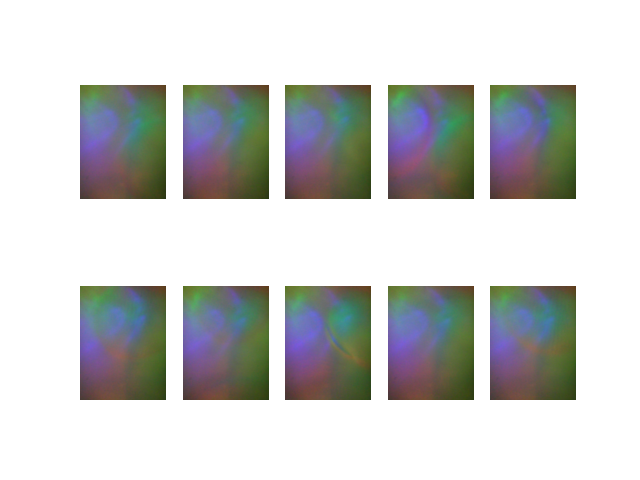
\includegraphics[scale=0.4]{docs/Project Report/Media/digit_frames.png}
    \caption{DIGIT tactile readings of 10 random examples}
    \label{fig:digit\_readings}
\end{figure}

\subsection{Developing a Pybullet Simulation for the Real Robot Setup}
Pybullet \cite{pybullet} is a physics engine and simulator designed to be used in robotics, machine learning and computer graphics. It is a Python wrapper for the Bullet Physics Library, which is an open-source physics engine that can simulate rigid body dynamics, soft body dynamics, and fluids.\\

I developed a Pybullet simulation alongside Jeffery Wei, a Master's project student with the Statistical Machine Learning Group as of writing this report. The simulation supports basic robot control and object manipulation, inverse kinematics and a tactile data collection pipeline.

\begin{figure}[H]
    \centering
    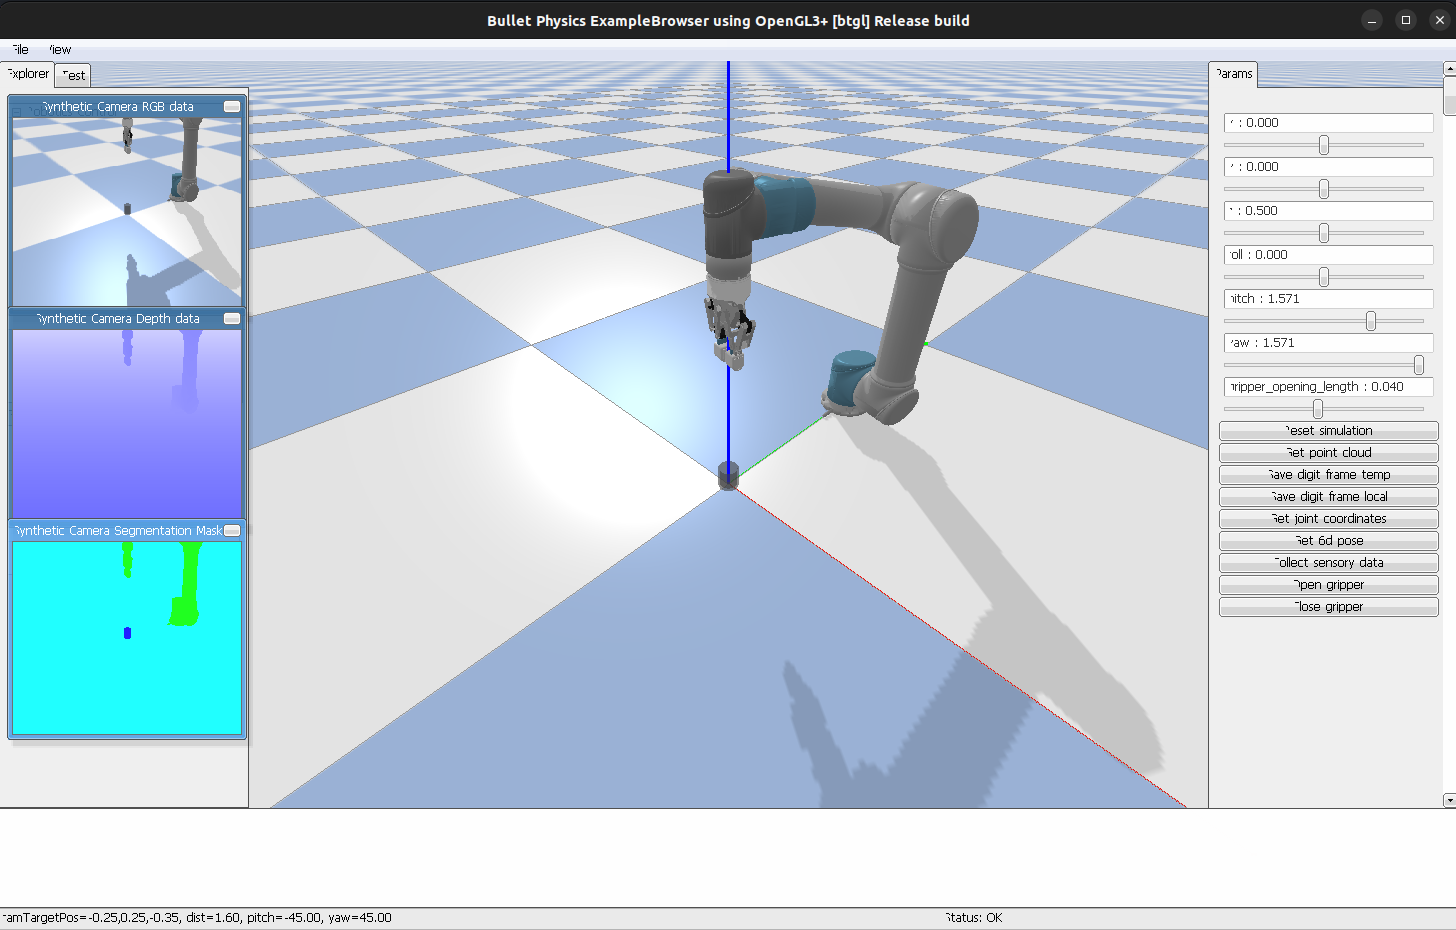
\includegraphics[scale=0.2]{docs/Project Report/Media/pybullet_sim.png}
    \caption{Screenshot of Pybullet Simulation for the Project}
    \label{fig:pb_sim_eg}
\end{figure}


%----------------------------------------------------------------------------------
% Section 2: Literature Review
% Focuses on important terms used throughout the report & academic papers read in-depth
%----------------------------------------------------------------------------------
\chapter{Background and Literature Review}
\label{chap:2}
\section{Robotic Regrasping}
\label{sec:2.1}
Robotic grasping requires precise coordination between the visual perception of the surrounding environment, efficient grasp planning and robustness in terms of the type of objects to grasp. 
\section{Academic Papers Reviewed in Depth}
\label{}
\subsection{More Than a Feeling: Learning to Grasp and Regrasp using Vision and Touch (Calandra et al)\cite{calandra}}
\label{}
\subsection{Generalizing Regrasping with Supervised Policy Learning (Hausman et al)\cite{hausman}}
\label{}
\subsection{Simultaneous Tactile Exploration and Grasp Refinement for Unknown Objects (Farias et al)\cite{farias}}
\label{}
\section{Conclusion on Literature Review}


%----------------------------------------------------------------------------------
% Section 3: Designing a Baseline Model and Deciding on Feature Representation of Tactile and Visual Data
%----------------------------------------------------------------------------------
\chapter{Baseline and Feature Representation Analysis}
\label{chap:3}
Mention the following:
- What common feature representations are there
- Results from your own testing
    - Collected tactile sensor readings (as tactile data) and end effector poses (as visual data)
    - Data was processed in 3 ways: raw, PCA with 3 main components, Convnet
    - Each type of processed data was then run with different feature combinations: tactile, vision \& tactile+vision
    - Display results
- Select the most promising representation and use it for actual generative model in Sec 4.


%----------------------------------------------------------------------------------
% Section 4: Actual Model
%----------------------------------------------------------------------------------
\chapter{Actual Model}
\label{chap:4}


%----------------------------------------------------------------------------------
% Section 5: Future Work
%----------------------------------------------------------------------------------
\chapter{Future Work}
\label{chap:5}
Since Pybullet is no longer being maintained, consider to move to mujico


%----------------------------------------------------------------------------------
% Appendix section
%----------------------------------------------------------------------------------
\appendix
\begin{thebibliography}{9}
\bibitem{haarnoja}
    Haarnoja, T., Zhou, A., Abbeel, P. & Levine, S..
    \textit{Soft Actor-CriticL Off-Policy Maximum Entroy Deep Reinforcement Learning with a Stochastic Actor, \href{https://arxiv.org/abs/1801.01290}{https://arxiv.org/abs/1801.01290}},
    ICML,
    2018roboti
\bibitem{nogueria}
    Nogueria et al,
    \textit{Unscented Bayesian Optimization for Safe Robot Grasping},
    IROS,
    2016
\bibitem{danielczuk}
    Danielczuk et al,
    \textit{Exploratory Grasping: Asymptotically Optimal Algorithms for Grasping Challenging Polyhedral Objects},
    2020
\bibitem{bekiroglu}
    Bekiroglu et al,
    \textit{Assessing Grasp Stability from Haptic Data},
    IEEE TRO,
    2011
\bibitem{frazier}
    Frazier,
    \textit{A Tutorial on Bayesian Optimization},
    2018
\bibitem{breyer}
    Breyer,
    \textit{\href{https://github.com/ethz-asl/vgn}{https://github.com/ethz-asl/vgn}}
    CORL,
    2020
\bibitem{calandra}
    Calandra et al,
    \textit{More Than a Feeling: Learning to Grasp and Regrasp using Vision and Touch},
    2018
\bibitem{hausman}
    Hausman et al,
    \textit{Generalizing Regrasping with Supervised Policy Learning},
    2017
\bibitem{farias}
    Farias et al,
    \textit{Simultaneous Tactile Exploration and Grasp Refinement for Unknown Objects},
    2021

\bibitem{digit}
    \href{https://digit.ml/}{DIGIT tactile sensors, 2020 @ Facebook}

\bibitem{pybullet}
    \href{https://pybullet.org/wordpress/}{Pybullet}

@article{Wang2022TACTO,
  author   = {Wang, Shaoxiong and Lambeta, Mike and Chou, Po-Wei and Calandra, Roberto},
  title    = {{TACTO}: A Fast, Flexible, and Open-source Simulator for High-resolution Vision-based Tactile Sensors},
  journal  = {IEEE Robotics and Automation Letters (RA-L)},
  year     = {2022},
  volume   = {7},
  number   = {2},
  pages    = {3930--3937},
  issn     = {2377-3766},
  doi      = {10.1109/LRA.2022.3146945},
  url      = {https://arxiv.org/abs/2012.08456},
}

\bibitem{franka}
    \href{https://www.franka.de}{Franka Emika}

\bibitem{robotiq}
    \href{https://robotiq.com/products/2f85-140-adaptive-robot-gripper}{Robotiq}

\end{thebibliography}

\chapter{Other appendices, e.g., code listing}
Put your appendix sections here
\end{document}

\end{document}